% GNUPLOT: LaTeX picture with Postscript
\begingroup
\footnotesize
  \makeatletter
  \providecommand\color[2][]{%
    \GenericError{(gnuplot) \space\space\space\@spaces}{%
      Package color not loaded in conjunction with
      terminal option `colourtext'%
    }{See the gnuplot documentation for explanation.%
    }{Either use 'blacktext' in gnuplot or load the package
      color.sty in LaTeX.}%
    \renewcommand\color[2][]{}%
  }%
  \providecommand\includegraphics[2][]{%
    \GenericError{(gnuplot) \space\space\space\@spaces}{%
      Package graphicx or graphics not loaded%
    }{See the gnuplot documentation for explanation.%
    }{The gnuplot epslatex terminal needs graphicx.sty or graphics.sty.}%
    \renewcommand\includegraphics[2][]{}%
  }%
  \providecommand\rotatebox[2]{#2}%
  \@ifundefined{ifGPcolor}{%
    \newif\ifGPcolor
    \GPcolortrue
  }{}%
  \@ifundefined{ifGPblacktext}{%
    \newif\ifGPblacktext
    \GPblacktexttrue
  }{}%
  % define a \g@addto@macro without @ in the name:
  \let\gplgaddtomacro\g@addto@macro
  % define empty templates for all commands taking text:
  \gdef\gplbacktext{}%
  \gdef\gplfronttext{}%
  \makeatother
  \ifGPblacktext
    % no textcolor at all
    \def\colorrgb#1{}%
    \def\colorgray#1{}%
  \else
    % gray or color?
    \ifGPcolor
      \def\colorrgb#1{\color[rgb]{#1}}%
      \def\colorgray#1{\color[gray]{#1}}%
      \expandafter\def\csname LTw\endcsname{\color{white}}%
      \expandafter\def\csname LTb\endcsname{\color{black}}%
      \expandafter\def\csname LTa\endcsname{\color{black}}%
      \expandafter\def\csname LT0\endcsname{\color[rgb]{1,0,0}}%
      \expandafter\def\csname LT1\endcsname{\color[rgb]{0,1,0}}%
      \expandafter\def\csname LT2\endcsname{\color[rgb]{0,0,1}}%
      \expandafter\def\csname LT3\endcsname{\color[rgb]{1,0,1}}%
      \expandafter\def\csname LT4\endcsname{\color[rgb]{0,1,1}}%
      \expandafter\def\csname LT5\endcsname{\color[rgb]{1,1,0}}%
      \expandafter\def\csname LT6\endcsname{\color[rgb]{0,0,0}}%
      \expandafter\def\csname LT7\endcsname{\color[rgb]{1,0.3,0}}%
      \expandafter\def\csname LT8\endcsname{\color[rgb]{0.5,0.5,0.5}}%
    \else
      % gray
      \def\colorrgb#1{\color{black}}%
      \def\colorgray#1{\color[gray]{#1}}%
      \expandafter\def\csname LTw\endcsname{\color{white}}%
      \expandafter\def\csname LTb\endcsname{\color{black}}%
      \expandafter\def\csname LTa\endcsname{\color{black}}%
      \expandafter\def\csname LT0\endcsname{\color{black}}%
      \expandafter\def\csname LT1\endcsname{\color{black}}%
      \expandafter\def\csname LT2\endcsname{\color{black}}%
      \expandafter\def\csname LT3\endcsname{\color{black}}%
      \expandafter\def\csname LT4\endcsname{\color{black}}%
      \expandafter\def\csname LT5\endcsname{\color{black}}%
      \expandafter\def\csname LT6\endcsname{\color{black}}%
      \expandafter\def\csname LT7\endcsname{\color{black}}%
      \expandafter\def\csname LT8\endcsname{\color{black}}%
    \fi
  \fi
  \setlength{\unitlength}{0.0500bp}%
  \begin{picture}(7200.00,5040.00)%
    \gplgaddtomacro\gplbacktext{%
      \csname LTb\endcsname%
      \put(3974,1764){\makebox(0,0){\strut{}-1}}%
      \put(3690,1507){\makebox(0,0){\strut{}-0.5}}%
      \put(3406,1250){\makebox(0,0){\strut{} 0}}%
      \put(3122,992){\makebox(0,0){\strut{} 0.5}}%
      \put(2838,735){\makebox(0,0){\strut{} 1}}%
      \put(697,1285){\makebox(0,0){\strut{}-2}}%
      \put(943,1210){\makebox(0,0){\strut{}-1.5}}%
      \put(1189,1136){\makebox(0,0){\strut{}-1}}%
      \put(1435,1062){\makebox(0,0){\strut{}-0.5}}%
      \put(1681,988){\makebox(0,0){\strut{} 0}}%
      \put(1927,913){\makebox(0,0){\strut{} 0.5}}%
      \put(2172,839){\makebox(0,0){\strut{} 1}}%
      \put(2417,765){\makebox(0,0){\strut{} 1.5}}%
      \put(2663,691){\makebox(0,0){\strut{} 2}}%
      \put(637,2070){\makebox(0,0)[r]{\strut{} 0}}%
      \put(637,2344){\makebox(0,0)[r]{\strut{} 5}}%
      \put(637,2619){\makebox(0,0)[r]{\strut{} 10}}%
      \put(637,2892){\makebox(0,0)[r]{\strut{} 15}}%
      \put(637,3167){\makebox(0,0)[r]{\strut{} 20}}%
      \put(637,3441){\makebox(0,0)[r]{\strut{} 25}}%
      \csname LTb\endcsname%
      \put(480,2499){\makebox(0,0){\strut{}$z$}}%
    }%
    \gplgaddtomacro\gplfronttext{%
      \put(5776,4316){\makebox(0,0)[r]{\strut{}$2*x**2 + y**2$}}%
      \csname LTb\endcsname%
      \put(5776,4096){\makebox(0,0)[r]{\strut{}       6}}%
      \csname LTb\endcsname%
      \put(5776,3876){\makebox(0,0)[r]{\strut{}       5}}%
      \csname LTb\endcsname%
      \put(5776,3656){\makebox(0,0)[r]{\strut{}       4}}%
      \csname LTb\endcsname%
      \put(5776,3436){\makebox(0,0)[r]{\strut{}       3}}%
      \csname LTb\endcsname%
      \put(5776,3216){\makebox(0,0)[r]{\strut{}       2}}%
      \csname LTb\endcsname%
      \put(5776,2996){\makebox(0,0)[r]{\strut{}       1}}%
      \csname LTb\endcsname%
      \put(5776,2776){\makebox(0,0)[r]{\strut{}exp$(x+y)$}}%
      \csname LTb\endcsname%
      \put(5776,2556){\makebox(0,0)[r]{\strut{}      20}}%
      \csname LTb\endcsname%
      \put(5776,2336){\makebox(0,0)[r]{\strut{}      15}}%
      \csname LTb\endcsname%
      \put(5776,2116){\makebox(0,0)[r]{\strut{}      10}}%
      \csname LTb\endcsname%
      \put(5776,1896){\makebox(0,0)[r]{\strut{}       5}}%
      \csname LTb\endcsname%
      \put(3789,1156){\makebox(0,0){\strut{}$x$}}%
      \put(1463,830){\makebox(0,0){\strut{}$y$}}%
      \csname LTb\endcsname%
      \put(480,2499){\makebox(0,0){\strut{}$z$}}%
    }%
    \gplbacktext
    \put(0,0){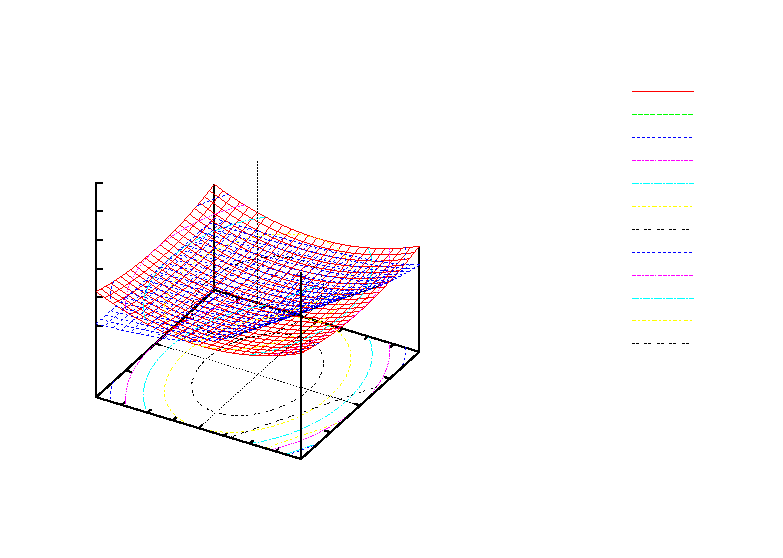
\includegraphics{appc2}}%
    \gplfronttext
  \end{picture}%
\endgroup
